
\section{Experiment}
\par An experiment was carried out at California Polytechnic State University to test the efficacy of habit-based educational software. We created a web-based application called \textit{Polycommit} that we connected to 4 college classes: \textbf{Introduction to Computer Networks}, \textbf{Introduction to Computer Graphics}, \textbf{Introduction to Computer Networks}, \textbf{Introduction to Operating Systems}, and \textbf{Linear Analysis I}. These classes were selected because they generally had subject matter that was easy to convert into online quizzes. For instance, one staple Linear Analysis problem is to find the determinant of a matrix, which is easy to input into an online form.

\par We presented Polycommit to each of the courses in the first 2 weeks of class. Students voluntarily sign up through a website hosted at https://polycommit.com/, where they can log in with one click through the main Cal Poly portal. This lets students easily access the website, while also guaranteeing that only Cal Poly students can sign up for the program.

\subsection{UI Overview}
\par Upon logging in, students click "Enroll" for the classes they wish to participate in. After enrolling, students can begin answering questions. There are two main "scores" that students earn by answering questions: \textbf{Commitment} and \textbf{Points}.

\par Commitment is a numerical value that represents how many \textit{unique} days a student has answered a question on the website. Students can earn up to 1\% extra credit on their final grade in the class by getting 15 Commitment.

\par Points are earned by answering questions. More points are awarded for correct answers, and bonus points are awarded based on the user's current Commitment. All participants in the experiment were placed in a raffle for \$20 Amazon gift cards. Additional entries into the raffle were awarded by earning more points.

\begin{figure*}
	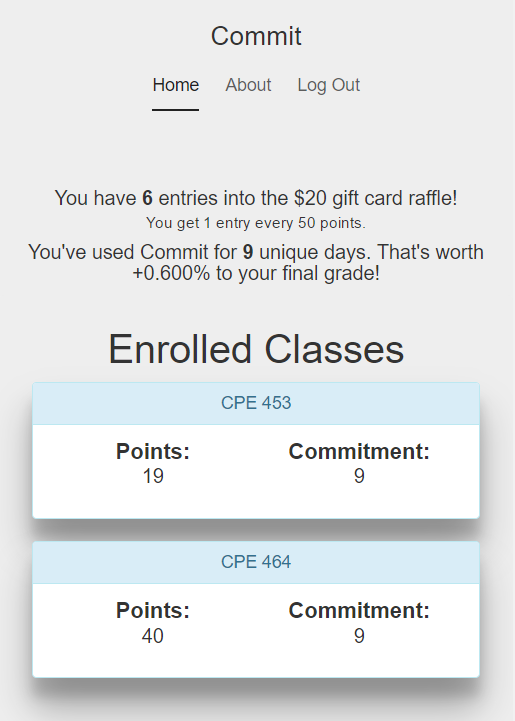
\includegraphics{figures/polycommit-screen}
	\caption{The "Home" screen for Polycommit. Students can see their current progress and can click on a course to answer challenges.}
	\label{fig:polycommit1}
\end{figure*}